\documentclass[11pt]{article}
\usepackage[margin=1in]{geometry}
\usepackage{indentfirst}
\usepackage[numbers,sort&compress]{natbib}
\usepackage{amsmath,amssymb,amsthm}
\usepackage{graphicx}
\usepackage[hidelinks]{hyperref}

\newtheorem{theorem}{Theorem}
\newcommand{\Z}{\mathbb{Z}}
\newcommand{\one}{\mathbf{1}}
\newcommand{\qminus}{q_-}
\newcommand{\qplus}{q_+}

\title{Pointwise Bounds on the Number of Rubik's Snake Shapes}
\author{Dmytro Fedoriaka}
\date{\today}

\begin{document}
\maketitle

\begin{abstract}
Let $S_n$ count the collision-free configurations of an oriented
$n$-wedge Rubik's Snake. For every $n\geq1$, we prove
$(3.45056)^{n-1}\leq S_n\leq
2.95621(3.66179)^{n-1}$. The proof is formalized in Lean.
\end{abstract}

\section{Introduction}

Rubik's Snake is a puzzle toy invented by Ern\H{o} Rubik in
1981. It is a chain of congruent right isosceles triangular
prisms, called \emph{wedges}, joined at their square faces. Each joint
has four quarter-turn positions. We count configurations in which
wedge interiors do not overlap; boundary contact is allowed.
The original toy has 24 wedges, but here the length $n$ can be any
positive integer.

We distinguish the two ends and identify configurations only under
translation and proper rotation, not reflection or reversal. The
order of the wedges is retained, even if two chains occupy the same
union of solids. We count static configurations, without requiring
a collision-free motion from a starting shape. Under these conventions,
the count $S_n$ is OEIS A375865~\cite{oeisA375865}.
The number of configurations for the original toy is
$S_{24}=13446591920995$
and was first computed in \cite{aylett2011}.


Rotation-sequence descriptions and geometric design methods appear
in~\cite{li2020,soul2022}. Related work studies periodic and palindromic
snakes~\cite{palindromic2021}, geometric structures~\cite{chen2023},
and planar configurations~\cite{grotto2024}.

This paper explains two pointwise bounds: a lower bound obtained by
joining many short, collision-free pieces, and an upper bound obtained
by remembering only a limited part of a snake's history. Put
\[
 \qminus=3.45056,\qquad \qplus=3.66179.
\]
We prove $\qminus^{n-1}\leq S_n$ and
$S_n\leq2.95621\qplus^{n-1}$ for every positive $n$.
All decimal constants in these statements are exact.
The construction ideas and the passage from finite certificates to
arbitrary lengths are described here; the geometric details and finite
checks are formalized in Lean.

The methods are related to those used for self-avoiding lattice walks.
Submultiplicative counting arguments go back to
Hammersley~\cite{hammersley1957}; lower-bound constructions and restricted
walk families are studied in~\cite{hara1993,bacher2011}, and finite-memory
upper bounds in~\cite{alm1993,noonan1998,ponitz2000,he2025}.
Other constrained walk counts, such as OEIS A336662 on the Manhattan
lattice~\cite{oeisA336662}, concern different local rules. For a snake,
successive directions must be perpendicular, but two complementary
wedges may share a cube. The constructions below use these rules
directly.

\section{Geometric model}\label{sec:geometry}

Write $e_x,e_y,e_z$ for the coordinate unit vectors and put
$\mathcal D=\{\pm e_x,\pm e_y,\pm e_z\}$.
For $p\in\Z^3$, let $Q_p=p+[-1/2,1/2]^3$.
If $a,b\in\mathcal D$ are perpendicular, define
\begin{equation}\label{eq:wedge}
 W(p;a,b)=\{u\in Q_p:(a+b)\cdot(u-p)\geq0\}.
\end{equation}
This is a wedge of volume $1/2$, with square-face normals $a,b$.
Their order records the entrance and exit faces.

\subsection{Rotation words}

Fix the first wedge. A configuration with $n$ wedges is then specified
by a word $r_1\cdots r_{n-1}$ over $\{0,1,2,3\}$, recording the
quarter turns at its joints. To recover its geometry, put
$p_0=0$, $d_0=e_y$, $d_1=e_x$, and, for $1\leq i<n$, set
\begin{equation}\label{eq:directions}
 d_{i+1}=R_{d_i}(r_i\pi/2)d_{i-1},\qquad
 p_i=p_{i-1}+d_i,
\end{equation}
where $R_d$ is right-handed rotation about the oriented axis $d$.
Wedge $i$, indexed from zero, is $W(p_i;-d_i,d_{i+1})$.
The vectors $d_0$ and $d_n$ also specify the free faces at the ends.
In particular, the last rotation determines the last wedge's
orientation, not a further center displacement. A center path alone
would lose this information.

A word is \emph{valid} if its wedge interiors are pairwise disjoint.
We write
\[
 a_k=S_{k+1}
\]
for the number of valid words with $k$ rotations. Thus $a_0=S_1=1$
and $a_k\leq4^k$.
Every contiguous subword of a valid word is valid: deleting wedges
cannot create a collision, and a rigid change of frame restores the
fixed initial wedge.

\subsection{An integer collision test}

Wedges in different lattice cubes have disjoint interiors.
Within one cube, $W(p;-a,-b)$ is the complement of $W(p;a,b)$ up to
their common boundary. No third wedge can share that cube without
overlapping another wedge's interior: two disjoint half-volume wedges fill it,
so their cutting planes must coincide.

Consequently, a visit with incoming direction $d$ and outgoing
direction $e$ occupies the unordered face pair $\{-d,e\}$.
A second visit to the same cube is legal exactly when its face pair
is the negative of the first. A third visit is never legal.
This rule reduces collision detection to lattice coordinates and
face directions, with no floating-point geometry.

\section{Lower bounds}\label{sec:lower}

The lower bound comes from a family of valid pieces that can be
joined freely. Two properties are essential. Joining pieces must
not introduce collisions, and different sequences of pieces must
give different rotation words. Otherwise, multiplying the numbers
of choices would overcount.

\subsection{Bridges and unique decomposition}

An \emph{x-bridge} enters its first cube at $(0,0,0)$ in direction
$+e_x$, occupies only layers $0\leq x\leq d-1$ for some $d>0$,
and leaves its last cube in direction $+e_x$ into layer $x=d$.
Its length $j$ is the number of occupied wedges, equivalently the
number of internal center steps plus the exit step.
Translate the next bridge so that it starts at this exit.
The two bridges occupy disjoint sets of $x$-layers, so they cannot
collide. Repeating this operation joins any sequence of bridges.
Prepending the fixed first wedge in the preceding layer turns a
sequence of total bridge length $k$ into a formula with $k$ rotations.

To make the sequence recoverable, we use only \emph{irreducible}
bridges. A forward crossing from layer $h$ to layer $h+1$ is a
\emph{separating cut} if every earlier occupied center has $x\leq h$
and every later one has $x\geq h+1$.
A bridge is irreducible when it has no such internal cut.
Cutting a concatenation at all separating cuts recovers precisely
its constituent irreducible bridges.

There is a convenient test for irreducibility. Each internal layer
boundary is crossed forward at least once. If it is never crossed
backwards, its forward crossing separates the bridge. If it is
crossed backwards, no forward crossing there can separate all earlier
and later centers. Thus a bridge is irreducible exactly when it
crosses every internal x boundary backwards at least once.
The enumeration records these crossings in a bit mask.

\subsection{A catalogue of short slab bridges}

The first part of our family is obtained by directly enumerating
irreducible $x$-bridges with progress values $d=1,2,3,4$ and at most
$20,20,18,21$ internal center steps, respectively. A depth-first
search extends a piece only when the directions are perpendicular,
the new wedge passes the collision test, and the path stays in its
slab. The backward-crossing mask selects the irreducible pieces.
Search pruning is allowed to discard pieces: for a lower bound,
an undercount is sufficient.

Only pieces whose first internal step is $+e_y$ need to be searched.
Rotating about the $x$-axis gives three more copies, starting with
$+e_z,-e_y,-e_z$. These four families are disjoint because their
first steps differ, and rotation preserves validity and all $x$-cuts.
This supplies four times as many bridges without four searches.
In particular, the catalogue contains bridges of lengths two and
three, which will ensure that every total length at least two is
available.

\subsection{Longer bridges assembled from transverse pieces}

To enlarge the catalogue without enumerating long bridges one by
one, we assemble them from short pieces in a transverse direction.
Fix $W\in\{2,3,4\}$ and keep all occupied centers inside
$0\leq x\leq W$. A new bridge has the form
\[
 \text{head}\;+\;\text{zero or more middle pieces}\;+\;\text{tail}.
\]
The whole object enters through $+e_x$ at $x=0$ and exits through
$+e_x$ from $x=W$, so its progress in $x$ is $W+1$.
The pieces are joined in the $+e_y$ direction.

The head exits above all of its occupied $y$-layers, although it may
dip below its entry layer. Each middle piece is an irreducible
$y$-bridge: it stays on or above its entry layer and strictly below
its exit layer. The tail stays on or above its entry layer, but may
rise above its final layer. These conditions place successive
pieces in disjoint $y$-layers. The head and tail can therefore
overhang their endpoints without colliding with neighboring pieces.

Separation also makes the pieces recoverable. We select heads with
no earlier separating exit followed by a $y$-bridge, and tails with
no initial $y$-bridge followed by a nonnegative suffix. Together with
irreducibility of the middle pieces, this means that cutting at
the transverse separating cuts gives a unique head--middle--tail
decomposition. Backward-crossing conditions certify these properties
in the short-piece search.

Only pieces of at most fourteen wedges are enumerated. Their occupied
$y$-spans are $0,1,2$; heads may enter at any layer of their span, while
middle pieces enter at the lowest layer. Tails are obtained by
reversing heads and applying a half-turn in $x$ and $y$. A head ending
at $x$-coordinate $E$ supplies a tail starting at $W-E$; its mask of
backward $x$-crossings is reflected accordingly.

Each piece is classified by its length, entry and exit x coordinates,
and backward x-crossing mask. This is enough information to count
assemblies by a finite recurrence. For a remaining length $r$,
entry coordinate $x$, and accumulated mask $m$, let $F(r,x,m)$
count continuations made of middle pieces followed by one tail.
If a middle-piece class $e$ has multiplicity $N_e$, length $\ell_e$,
exit coordinate $x_e$, and mask $m_e$, its contribution is
\[
 N_e F(r-\ell_e,x_e,m\mathbin{\mathrm{OR}}m_e).
\]
The recurrence sums these terms over classes entering at $x$ with
$\ell_e\leq r$ and adds tails of exactly the remaining length. A tail is accepted
only when the final mask includes every internal x cut.
Finally, summing over the head choices gives the total.
Lean checks a finite table of recurrence inequalities and proves
that it undercounts distinct geometric assemblies. There is no
need to list every long assembled bridge.

The complete mask makes each resulting x-bridge irreducible.
Its total displacement in $y$ is positive; a half-turn about the
$x$-axis produces
a disjoint second family with negative y displacement.
We keep assembled lengths up to $64$. For $W=2$ we keep only lengths
greater than $19$, and for $W=3$ only lengths greater than $22$,
avoiding overlap with the directly enumerated bridges of the same
x progress. For $W=4$, the x progress is new, so no such lower
cutoff is needed. The union of these families and the short slab
catalogue is therefore still duplicate-free.

\subsection{From the catalogue to the pointwise bound}

Let $c_j$ be the certified lower count of bridges of length $j$ in
the combined catalogue, for $1\leq j\leq64$. Let $A_k$ count
concatenations from this catalogue of total length $k$, with
$A_0=1$ and $A_k=0$ for negative $k$.
Collision freedom and unique decomposition give
\begin{equation}\label{eq:renewal}
 A_k\geq\sum_{j=1}^{64}c_jA_{k-j}\quad(k\geq1),
 \qquad A_k\leq a_k.
\end{equation}
The first inequality follows by choosing the first bridge and then the
remaining concatenation. The second embeds each concatenation into a valid
formula.

For an exponential sequence $\qminus^k$ to satisfy the same lower
recurrence, we need
\begin{equation}\label{eq:lower-polynomial}
 \qminus^{64}\leq\sum_{j=1}^{64}c_j\qminus^{64-j}.
\end{equation}
The Lean development verifies the stronger inequality at
$r_-=17252837/5000000$ using integers:
\[
 17252837^{64}\leq
 \sum_{j=1}^{64}c_j\,17252837^{64-j}\,5000000^j.
\]
Since $\qminus<r_-$ and the $c_j$ are nonnegative, dividing by
$r_-^{64}$ shows that this inequality implies
\eqref{eq:lower-polynomial}. No approximate root calculation is needed.

\begin{theorem}\label{thm:lower}
For every positive integer $n$,
\[
 S_n\geq(3.45056)^{n-1}.
\]
\end{theorem}
\begin{proof}
We first obtain a lower bound with a fixed positive prefactor.
The length-two and length-three bridges give $A_k\geq1$ for all
$k\geq2$. Set $C=4^{-66}$. Since $\qminus<4$, we have
$C\qminus^k\leq1\leq A_k$ for $2\leq k\leq65$.
For $k\geq66$, induction using \eqref{eq:renewal} and
\eqref{eq:lower-polynomial} gives
\[
 A_k\geq C\sum_{j=1}^{64}c_j\qminus^{k-j}
 \geq C\qminus^k.
\]
It follows that $a_k\geq C\qminus^k$ for all $k\geq0$;
the cases $k=0,1$ follow from $a_k\geq1$.

To remove $C$, split any valid word of length $p+q$ into its two
valid subwords. The pair determines the original word, hence
\begin{equation}\label{eq:submultiplicative}
 a_{p+q}\leq a_pa_q.
\end{equation}
For fixed $k\geq1$ and any positive integer $m$, this gives
\[
 C\qminus^{mk}\leq a_{mk}\leq a_k^m,
 \qquad
 a_k\geq C^{1/m}\qminus^k.
\]
Letting $m\to\infty$ yields $a_k\geq\qminus^k$.
The case $k=0$ is equality. Substituting $k=n-1$ proves the claim.
\end{proof}

\section{Upper bounds}\label{sec:upper}

For the upper bound we deliberately count too many words. A finite
automaton remembers only a suffix of the rotation history, enough
to detect many short collisions. It may miss collisions involving
older wedges, but it must accept every valid formula. An exact
weight inequality then bounds its number of paths at every length.

\subsection{Remembering short collision patterns}

A \emph{minimal collision word} is invalid, but its prefix and suffix
of one fewer symbol are both valid. Its only collision is between
its first and last wedges. We search for such words of rotation
lengths $4,6,8,10,12,14,16$. These are even lengths because the
first and last centers must coincide, and each center step changes
the parity of the sum of the coordinates.
The computation produces $4\,441\,614$ collision words.

Let $\mathcal P$ be the dictionary of all their proper prefixes,
including the empty word. It is prefix-closed. After reading a
word $u$, retain only $p(u)$, its longest suffix belonging to
$\mathcal P$. This is the part of the history that might still
complete one of the recorded collision patterns.
For example, if the longest relevant ending is $321$, a much
longer history ending in $0321$ can be replaced by the state $321$.

Given a state $v$ and a new symbol $r$, we test the short word $vr$
geometrically. We reject the transition if it is invalid; otherwise,
we move to $p(vr)$. Prefix closure ensures that
\[
 p(ur)=p\bigl(p(u)r\bigr),
\]
so the update does not need the discarded history.
Indeed, removing the last symbol from a nonempty dictionary suffix
of $ur$ leaves a dictionary suffix of $u$.

Every valid formula follows a path from the empty state:
each short word tested along the way is a suffix of an actual
valid prefix. Conversely, some paths may describe invalid formulas,
because their collisions were forgotten. Thus the path count is
an upper bound, not an exact count. The argument needs prefix
closure and the geometric transition test; it does not require the
collision search to find every possible short pattern.

The resulting graph has $4\,748\,260$ states and $14\,133\,721$
rotation-labeled edges. Define the outgoing operator
\[
 (Tf)(v)=\sum_{v\xrightarrow{r}u}f(u).
\]
Different labels are counted separately even when they have the
same target. With $\one$ the all-ones function and $\varnothing$
the empty state, the number of accepted words of length $k$ is
$(T^k\one)(\varnothing)$. Therefore
\begin{equation}\label{eq:path-upper}
 a_k\leq(T^k\one)(\varnothing).
\end{equation}

\subsection{A weight certificate and six terminal steps}

Assign each state a nonnegative integer weight $w(v)$.
The main certificate checks
\begin{equation}\label{eq:upper-weight}
 10^9Tw\leq3661786723w.
\end{equation}
Since $3661786723/10^9<\qplus$, this implies $Tw\leq\qplus w$
at every state. Iterating gives $T^kw\leq\qplus^kw$.
The weights are generated by starting with $w_0=10^{18}\one$
and taking 48 componentwise integer updates
\[
 w_{i+1}=\left\lfloor Tw_i/4\right\rfloor.
\]
This procedure only proposes the weights; the separate exact check
\eqref{eq:upper-weight} is what certifies them.

Weights alone need not compare well with the all-ones function.
In particular, a state with no long continuation may have weight
zero. Instead of forcing every weight to be positive, count the
last six steps explicitly. Starting with $\one$, six applications
of $T$ give the exact continuation counts $T^6\one$.
The certificate verifies
\begin{equation}\label{eq:terminal}
 sT^6\one\leq w,\qquad s=2\,990\,000\,000\,000,
\end{equation}
as well as
\[
 w(\varnothing)=21\,309\,021\,059\,784\,288.
\]
Zero weights are harmless: \eqref{eq:terminal} ensures that such
states cannot support a six-step continuation.
All these comparisons use integers, not a floating-point spectral
estimate.

\begin{theorem}\label{thm:upper}
For every positive integer $n$,
\[
 S_n\leq2.95621(3.66179)^{n-1}.
\]
\end{theorem}
\begin{proof}
For $k\geq6$, apply \eqref{eq:terminal} to the last six steps,
then \eqref{eq:upper-weight} to the preceding steps:
\[
 a_k\leq(T^k\one)(\varnothing)
 \leq s^{-1}(T^{k-6}w)(\varnothing)
 \leq s^{-1}\qplus^{k-6}w(\varnothing).
\]
The exact numerical check
\[
 \frac{21\,309\,021\,059\,784\,288}
 {2\,990\,000\,000\,000\,\qplus^6}\leq2.95621
\]
gives $a_k\leq2.95621\qplus^k$.
For $k=0,\ldots,5$, each of the six inequalities
$4^k\leq2.95621\qplus^k$ is checked directly, so the elementary
bound $a_k\leq4^k$ covers the remaining cases.
Again, $k=n-1$ gives the result.
\end{proof}

\section{Conclusion}

For every positive number of wedges, the two constructions give
\begin{equation}\label{eq:pointwise-bounds}
 \boxed{(3.45056)^{n-1}\leq S_n\leq
 2.95621(3.66179)^{n-1}.}
\end{equation}
The lower bound counts a restricted family whose pieces join
without collisions and can be uniquely recovered. The upper
bound counts a larger language whose finite memory may overlook
collisions. Finite recurrence and state-weight certificates turn
these two constructions into bounds for all lengths.

Figure~\ref{fig:bounds-comparison} compares the bounds with the exact
counts through $n=28$. The three curves track one another closely
on a logarithmic scale, over more than fifteen orders of magnitude.
For example, at $n=28$ the upper bound is about $2.06$ times $S_{28}$,
while the lower bound is about $S_{28}/7.13$.

\textbf{Lean formalization.} The complete formalized proofs are available at
\begin{center}
 \url{https://github.com/fedimser/rubiks-snake-lean}.
\end{center}

The final results, using higher decimal precision, are in
\href{https://github.com/fedimser/rubiks-snake-lean/blob/master/lean/RubiksSnake/SnAsymptotic/FinalResults.lean}
{\texttt{FinalResults.lean}}.

The lower-bound certificate is in
\href{https://github.com/fedimser/rubiks-snake-lean/blob/master/lean/RubiksSnake/SnAsymptotic/CapCandidateCertificate.lean}
{\texttt{CapCandidateCertificate.lean}}.

The upper-bound certificate is in
\href{https://github.com/fedimser/rubiks-snake-lean/blob/master/lean/RubiksSnake/SnAsymptotic/ForbiddenPrefixSixteenCertificate.lean}
{\texttt{ForbiddenPrefixSixteenCertificate.lean}}.

\textbf{Future work.}
The lower bound could be raised by expanding the certified bridge
catalogue. Enumerating longer or wider slab bridges, retaining more
classes of transverse pieces, and extending the range of assembled
lengths would increase the coefficients $c_j$ and might allow a larger
value of $\qminus$ in \eqref{eq:lower-polynomial}. The upper bound could
be lowered by recording longer minimal collision words or retaining
more geometric information in the automaton states, so that fewer
invalid formulas survive the finite-memory relaxation. A more targeted
search for state weights, possibly combined with a different number of
explicitly counted terminal steps, could also improve $\qplus$ or the
prefactor. These refinements would enlarge the finite enumerations and
certificates but would leave the overall proof strategy unchanged.

\textbf{Growth constant.} The submultiplicative inequality \eqref{eq:submultiplicative} implies,
by Fekete's lemma, that the exponential growth constant
$\mu=\lim_{n\to\infty}S_n^{1/(n-1)}$
exists. From \eqref{eq:pointwise-bounds}, it follows that
$3.45056\leq\mu\leq3.66179$.
It remains an open question whether $S_n=\Theta(\mu^{n-1})$.

\begin{figure}[!hb]
\centering
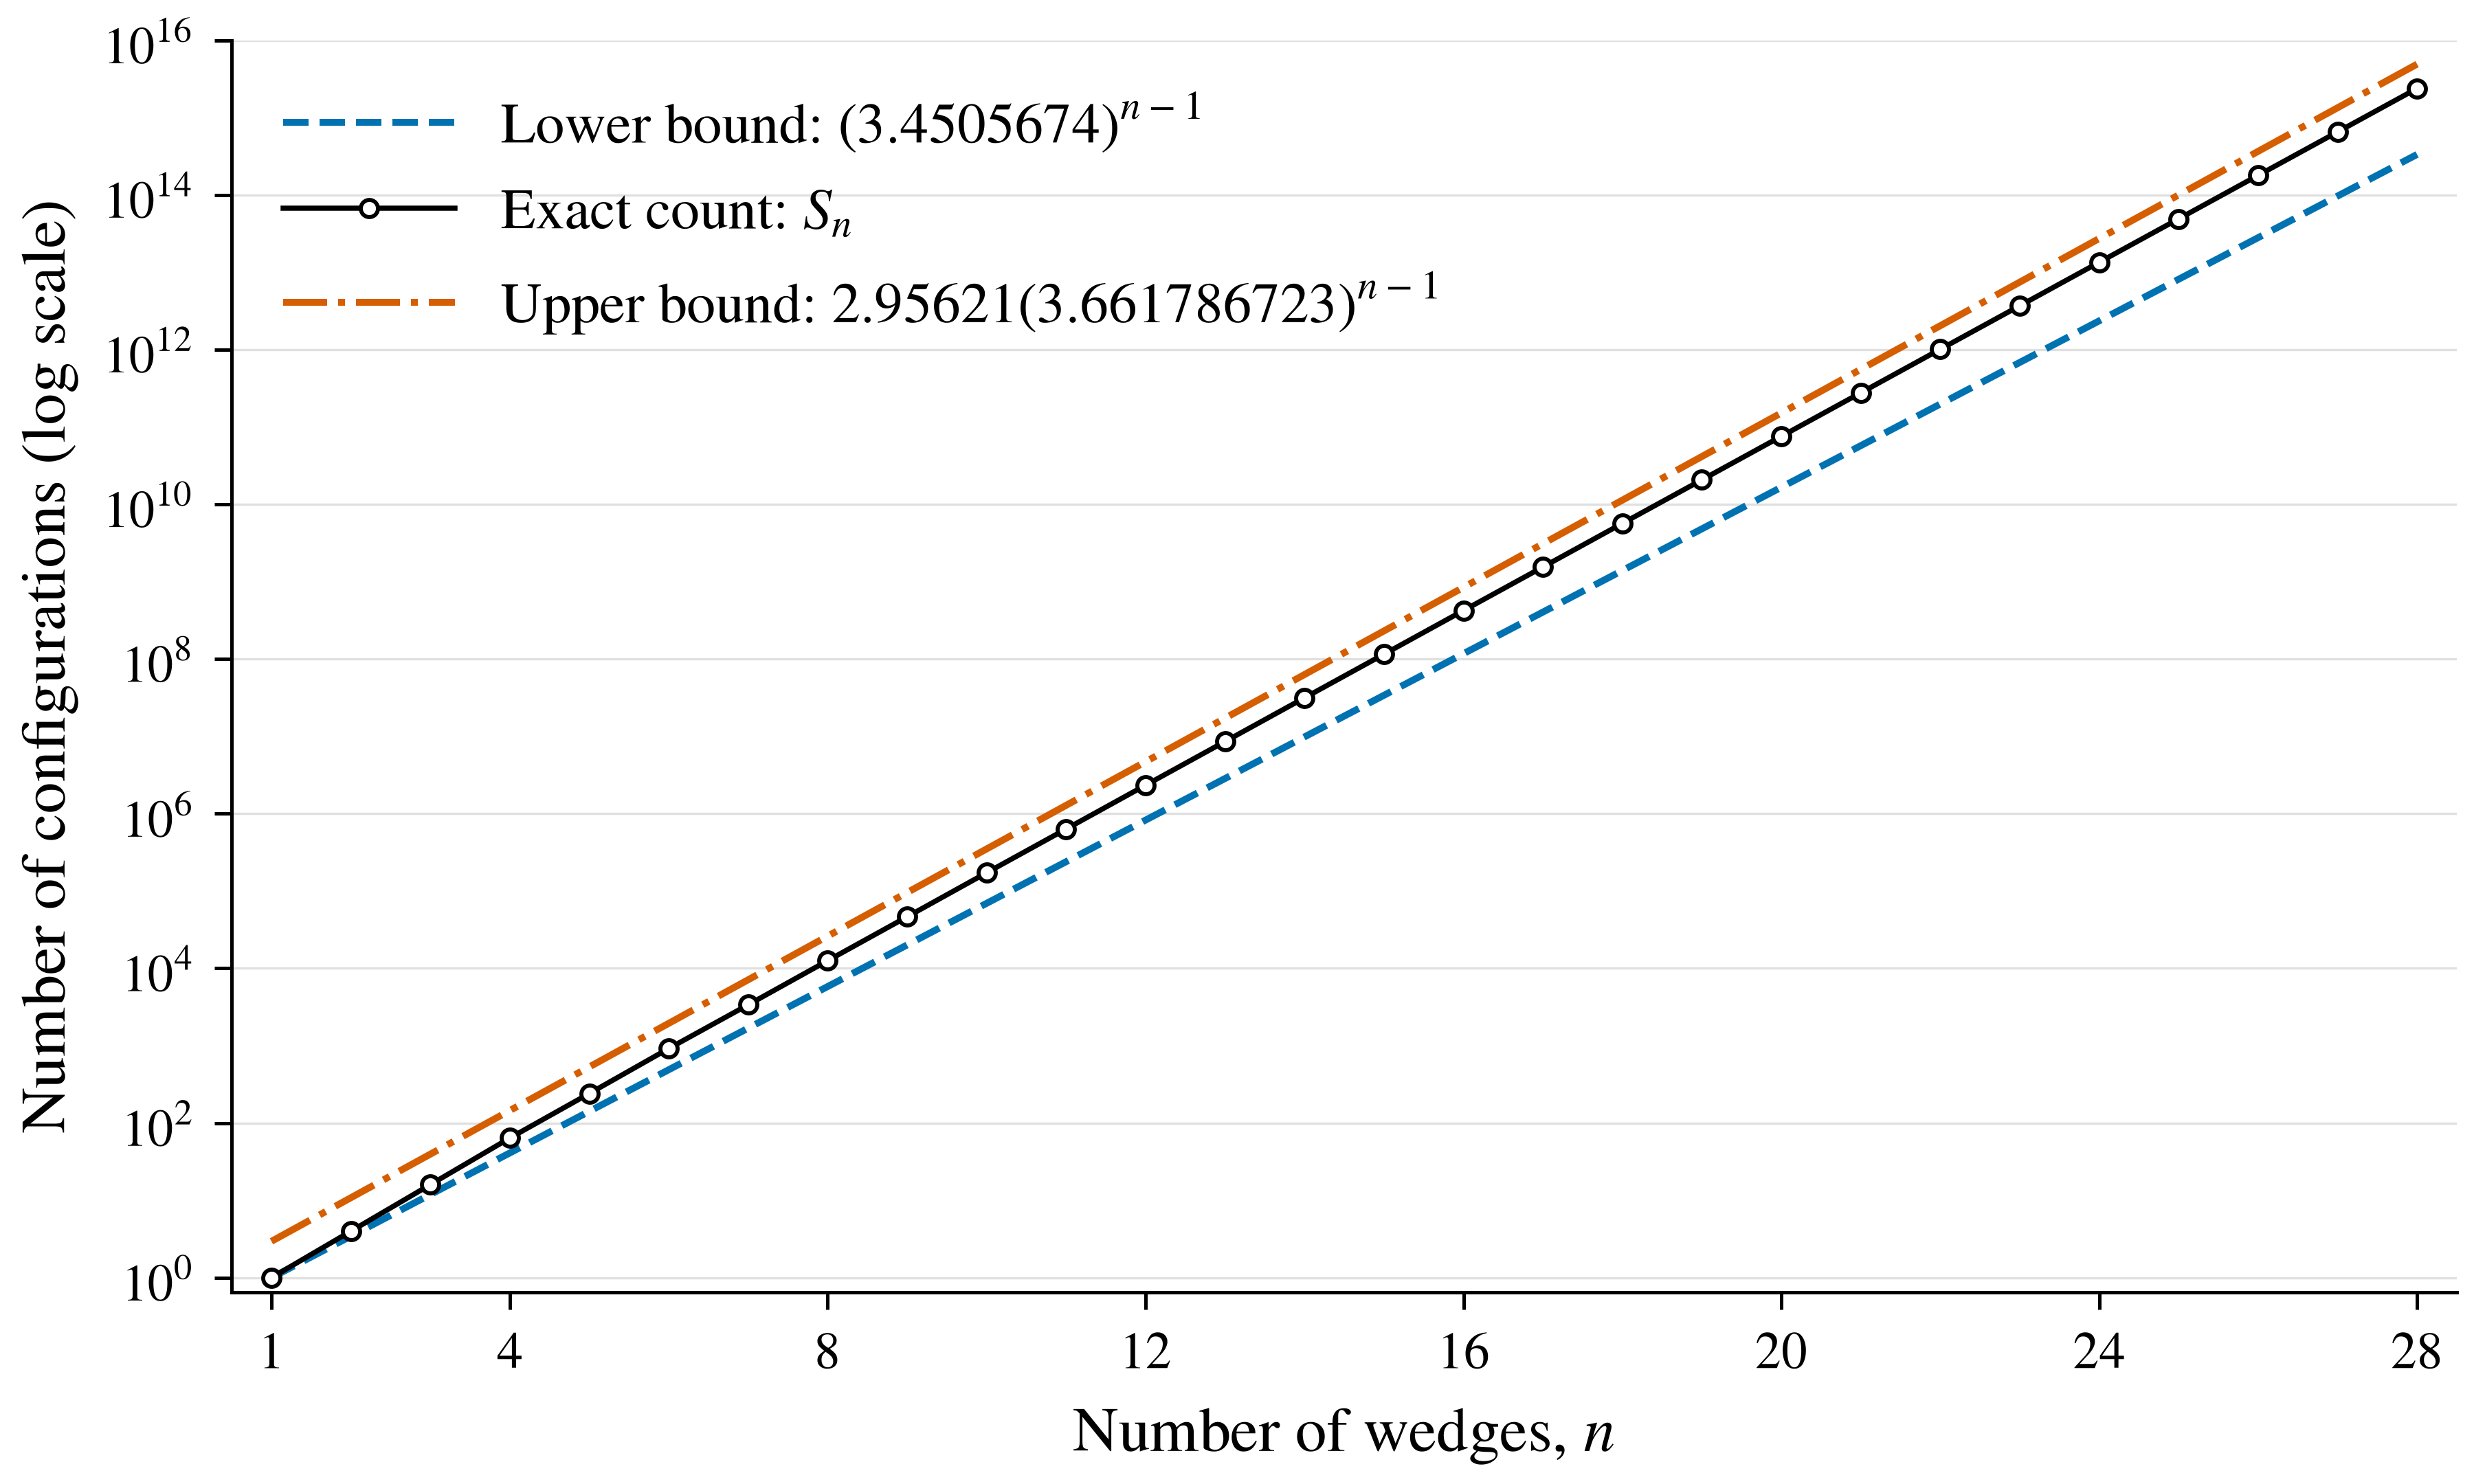
\includegraphics[width=0.95\linewidth]{bounds_plot.png}
\caption{Pointwise lower and upper bounds compared with
the exact counts $S_n$ for $1\leq n\leq28$.}
\label{fig:bounds-comparison}
\end{figure}

\clearpage
\bibliographystyle{plainnat}
\bibliography{refs}
\end{document}
